\chapter{Introduction}
\label{sec:Introduction}


%%%% Citation
%{\small
%\begin{flushright}
%"The problems of the world cannot possibly be solved by skeptics or cynics whose horizons are limited by the obvious realities. We need men who can dream of things that never were and ask why not?" \\ \emph{John F. Kennedy}
%\end{flushright}
%}
%\vspace{+10pt}
%%%%


In many robotic systems, actuators are often required to operate in distinctively different torque-speed load conditions. Machine tools, for instance, are usually either moving at high-speed unloaded during reaching phases, or moving slowly applying large forces during manufacturing operations (see Fig. \ref{fig:machinetool}). Also a legged robot, for example, has to move its leg forward quickly through the air and, once touching the ground, it has to bear a large load (see Fig. \ref{fig:leggedrobot}), or a gripper needs to reach the part quickly and then has to apply large holding forces (see Fig. \ref{fig:gripper}). These two operating conditions, high speed at low torque vs. high torque at low speed, are often an order of magnitude different, while the required output power is similarly low.

%
\begin{figure}[H]
				\vspace{-10pt}
        \centering
				\subfloat[Machine tool]{
				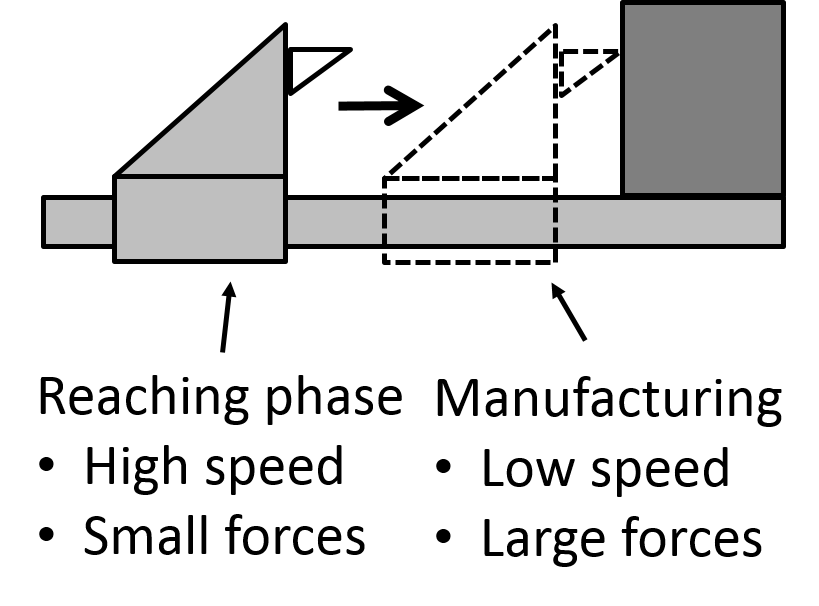
\includegraphics[width=0.30\textwidth]{machinetool.png}
				\label{fig:machinetool}}
        \subfloat[Legged robot]{
				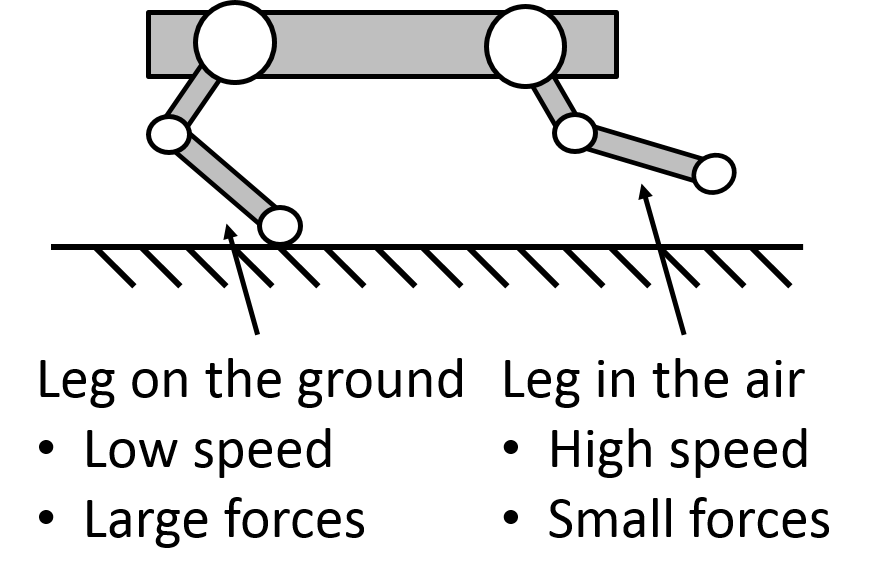
\includegraphics[width=0.30\textwidth]{leggedrobot.png}
				\label{fig:leggedrobot}}
				\subfloat[Gripper]{
				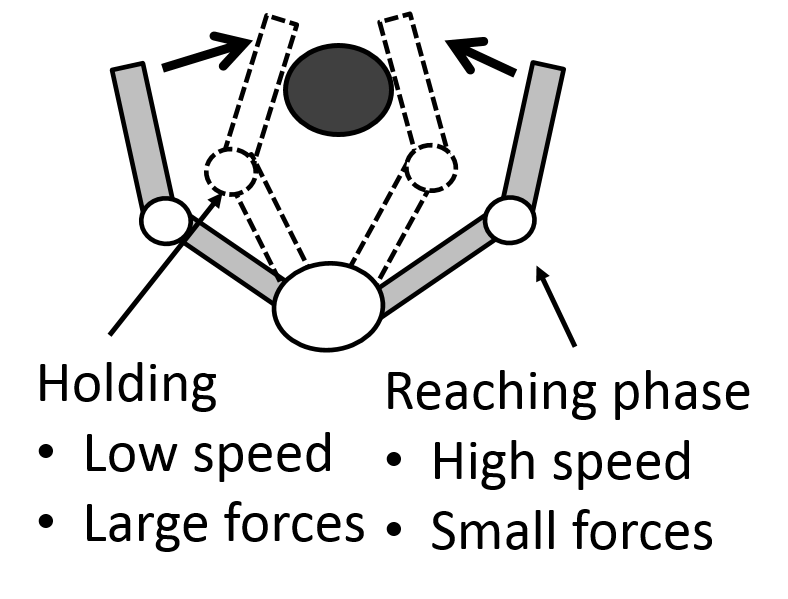
\includegraphics[width=0.30\textwidth]{gripper.png}
				\label{fig:gripper}}
        \caption{Robotics system encountering very different load situation}
				\label{fig:app}
\end{figure}

This discrepancy in requirements is problematic as most actuators will be operating far for their optimal conditions with a gear ratio picked from a middle ground. Electromagnetic actuators are not optimal in term of efficiency and power output at extremum torque-speed conditions. This often leads to the use of over-sized and inefficient actuators, which is inhibitory particularly for mobile robots.


\section{Limitation of traditional actuation systems}
\label{sec:limitationOfTraditionnalRoboticSystems}

Electric motor have a power efficiency of about 200 W/Kg

actuator review here

Traditional robots generally use actuators that behave as displacement-sources because of their high intrinsic impedance. These include geared EM motors and hydraulics cylinders. Using a force sensor, it is possible to control the output force using those actuators, but the bandwidth is rather limited. To guarantee the stability of the force-feedback scheme only half the intrinsic inertia can be canceled \cite{hogan_impedance_2004}. Since 70's, roboticists have been attempting to build actuators that can behave naturally as a force-source such as series-elastic actuators, pneumatic cylinder and air-muscles \cite{hanafusa_stable_1977}\cite{pratt_series_1995}. However, because of the physical limitation of compliant transmission materials, the achievable bandwidth is limited and precise position control is hardly achievable. Direct drive EM actuators are the best force-source actuators with high fidelity, high bandwidth. However, the very low force density and low efficiency at low speeds make them impractical for mobile robot applications \cite{hollerbach_comparative_1992}. Moreover, on the other hand, actuators with non-back-drivable mechanisms have the advantage for pure position control tasks and they can bear very large load without any power consumption.

Since both small and large intrinsic impedances are advantageous in different scenario, several group have developed variable intrinsic impedance actuators, such as based on variable stiffness spring \cite{tonietti_design_2005}, antagonist non-linear devices \cite{koganezawa_antagonistic_2006}, a series-compliance that can be locked with a brake \cite{leach_linear_2012} and dual-motors in serial configuration \cite{kim_serial-type_2010}. Furthermore, so-called macro-micro actuators, can improve the bandwidth of force-source type of actuators by exploiting the high-bandwidth of a small actuator in parallel, allowing for wider-range impedance control and improved position control \cite{morrell_parallel-coupled_1998}.

While the actuator work in robotics have been focused on impedance and bandwidth issues, in the powertrain field the torque-speed matching issue is predominant, since power density and efficiency are critical for mobile systems.


\section{Proposed approach: Variable Transmissions}
\label{sec:ProposedSolutionRobotsUsingMultipleGearRatioActuators}


To meet the power requirement of all operating points with small actuators, it is proposed to use electric motors coupled to a gearbox with two drastically different gear ratio, see Fig. \ref{fig:2s}. 

\begin{figure}[htb]
        \centering
				\subfloat[two drastically different reduction ratios]{
				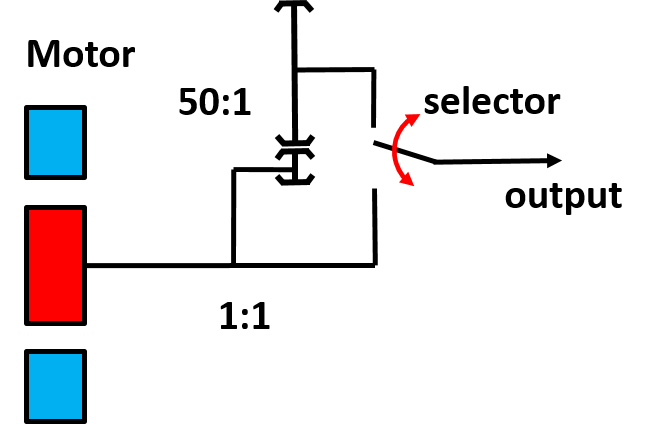
\includegraphics[width=0.35\textwidth]{2speed.png}}
        \subfloat[discrete operating modes]{
				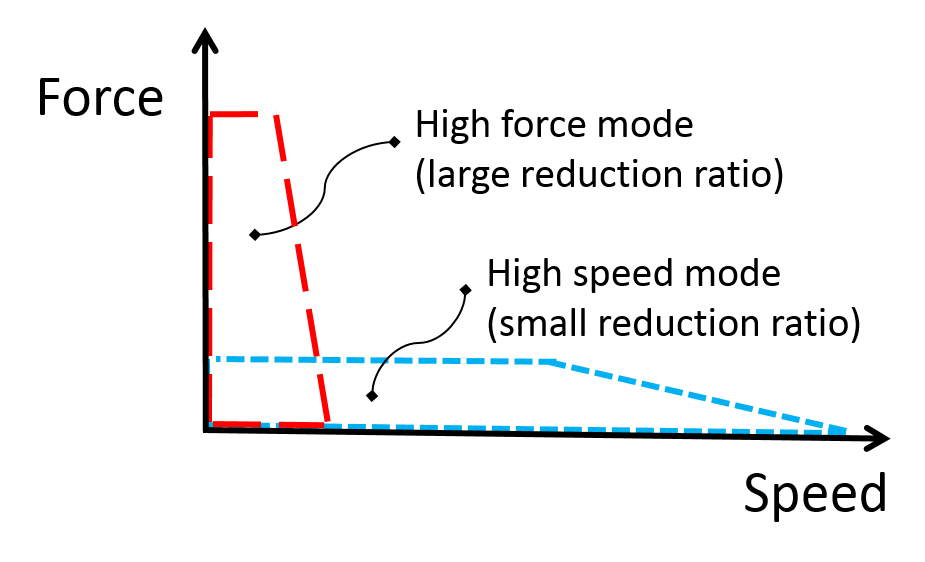
\includegraphics[width=0.40\textwidth]{1DOFmodes.png}}
        \caption{Dual-speed actuator}\label{fig:2s}
\end{figure}


The two main advantage of the approach are: \textbf{good power output and efficiency for a wide range of output speeds} and \textbf{radical changes of intrinsic impedance} (goes with the square of the reduction ratio). 

\subsection{Features of gear-shifting in a robotic context}

\paragraph{Power output and efficiency}
In many situation, using multiple gear ratios allows for the downsizing of the motors while still meeting required forces/speeds capabilities. Furthermore, by actively selecting gearing ratios to keep motors in efficient regimes, the energy consumption of a robot can be greatly reduced. 

\paragraph{Radical changes of intrinsic impedance}
The gearing ratio has a radical effect on the output impedance of a robot; the motor inertia and viscous damping are reflected to the output proportionally with the square of the gearing ratio. Gear-shifting can thus also be used as an alternative approach to variable impedance actuation. A two-speed actuator could be made back-drivable by selecting the small reduction ratio, to interact safely with the environment and to make use of the natural dynamic behavior of a robot.  Alternatively, a two-speed actuator could be made non-back-drivable by selecting the large reduction ratio, to rejected disturbances or to hold a weight without consuming power.


\begin{figure}[H]
	\centering
		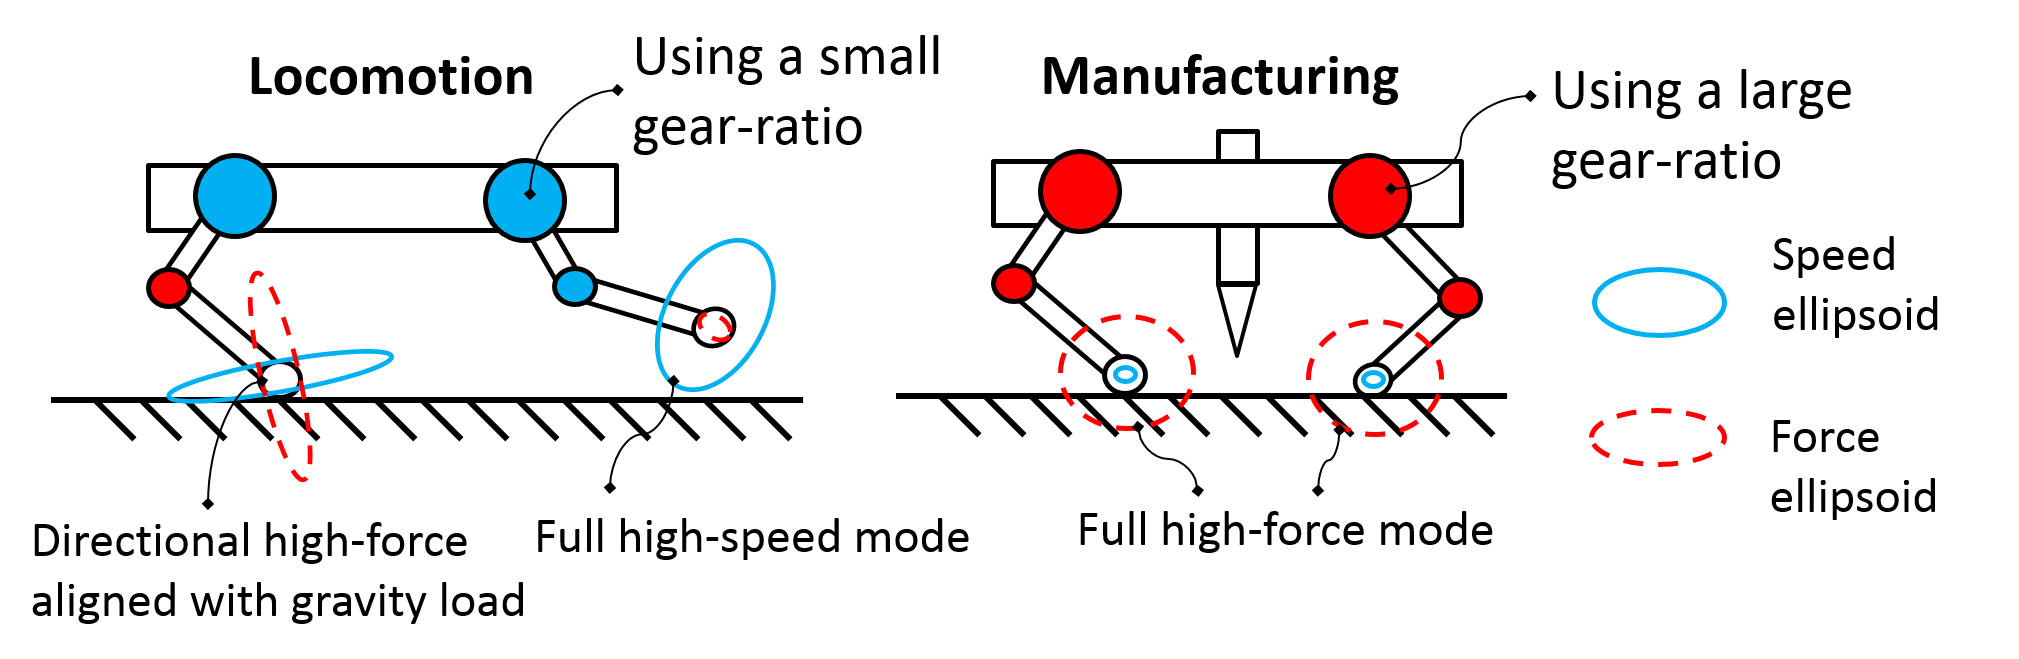
\includegraphics[width=0.90\textwidth]{gearselectionlegged.png}
	\caption{Example of advantageous gear selection with a multi-DOF robot}
	\label{fig:gearselectionlegged}
\end{figure}


\section{Main challenges}
\label{sec:MainChallenges}

\subsection{Actuator design}
\label{sec:ActuatorDesign}

\subsection{Control and planning of hybrid system}
\label{sec:ControlAndPlanningOfHybridSystem}



\section{Original contributions}
\label{sec:contribution}


\section{Organization of the thesis}
\label{sec:OrganisationOfTheThesis}




